% Proposal document for gattrib evolution
\documentclass[a4,10pt]{article}
\usepackage{graphicx}
\usepackage{url}
\usepackage{hyperref}
\title{Proposal for a new attribute sheet editor for gEDA}
\author{G.~D. Edwards}
\begin{document}
\maketitle
\section{Introduction}
It is proposed that a new spreadsheet-type attribute editor be added
to the gEDA/gaf suite to supplement and/or supercede the gattrib tool
currently shipping. Figure \ref{fig:wireframe} shows a mockup of the
UI.
\begin{figure}
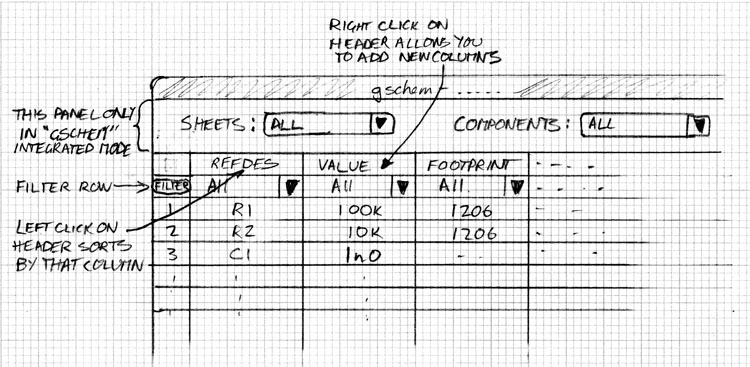
\includegraphics{gattrib_evolution_wireframe_150.jpg}
\caption{Wireframe of the attribute sheet editor}
\label{fig:wireframe}
\end{figure}
\section{Features}
The following features are proposed
\begin{itemize}

\item The attribute sheet editor will be useable as a non-modal window
  inside gschem.

\item The attribute sheet editor will also be useable as a standalone
  application (gattrib)

\item Sheet can be sorted by clicking on the top of any of the
  attribute columns, in the usual spreadsheet manner;

\item Sheet view can be filtered against unique values in each column;
  similar to spreadsheet filtering. This breaks down for refdes; I
  suggest this attribute is filtered/grouped by the prefix rather than
  the whole attribute value.

\end{itemize}
%
\section{Development Assumptions}
The following assumptions are held:
\begin{itemize}

\item The Gtksheet widget will not be used. It's not maintained and likely to
  stay that way.

\item No new dependencies will be introduced. This means that the
  sheet widget will have to be self-contained in the gEDA/gaf
  codebase.

\end{itemize}
\section{Issues and Questions}
\subsection{Open}
%
\subsubsection{Where should the code live?}
The sheet display code and (perhaps) to some extent the intermediate
data model will need to be used by both the gschem app and
gattrib. Can code that is in the .../gattrib/ tree be used by the
gschem application? Or should it be devolved into a separate
``libattribsheet'' library? GDE is fairly certain libgeda is not the
place for it due to the existence/amount of display code.
%
\subsubsection{Does it degeneralise gschem?}
Is there anything in this development that would threaten the
design/development flows of existing gschem users? Don't want to start
another gEDA-user holy war.

Unless it's justified.
%
\subsubsection{Does gattrib actually need to be replaced?}
I'm unsure what the current status of gattrib is. Bug
\href{https://sourceforge.net/tracker/?func=detail&atid=818426&aid=2832985&group_id=161080}{2832985}
seemed to suggest that gattrib would have difficulty building on
recent GTK+ code but Peter C committed a fix for this. Is this just a
sticking plaster or is it worthwhile persevering with the current
gattrib code?
%
\subsection{Resolved}

\end{document}
